\documentclass[a4paper, 12pt]{scrartcl}
\usepackage{scrpage2}
\usepackage[left=2.5cm,right=2.5cm, top=3cm, bottom=4cm]{geometry}
\usepackage[utf8]{inputenc}
\usepackage[ngerman]{babel}
\usepackage[T1]{fontenc}
\usepackage{amsmath}
\usepackage{amssymb}
\usepackage{amsfonts}

\usepackage{graphicx}

\usepackage{float}
\usepackage{adjustbox}
\usepackage{hyperref}
\usepackage{textcomp}
\usepackage{multirow}
\usepackage{array}

%\usepackage{enumerate}
\usepackage[shortlabels]{enumitem}

%Zeichnungen
\usepackage{tikz}
\usepackage[european]{circuitikz}

% Einrücken verhindern
\setlength{\parindent}{0em} 


\begin{document}

\begin{titlepage}
	\centering
	{\Huge\bfseries Versuchsprotokoll\par}
	\vspace{2cm}
	{\scshape\LARGE Wärmelehre \par}
	\vspace{1cm}
	{\Large Bestimmung des Adiabatenkoeffizients \\ mit der Rüchardt-Methode\par}
	\vfill
	{\large\itshape Simon Schwarz und Marius Ising\par}

	\vfill
\end{titlepage}

\tableofcontents
\newpage


\section{Gedämpfter LCR-Schwingkreis}


\subsection{Versuchsbeschreibung}

In einer Serienschaltung aus Spule $L$, Kondensator $C$ und Ohmschem Widerstand $R$ (vgl. Abb. \ref{abb:schaltLCR}) wird der Kondensator zunächst aufgeladen und anschließend die Spannungsquelle mit einem Taster überbrückt, sodass der Kondensator sich über den Widerstand entladen kann. Dabei entlädt sich der Kondensator nicht sofort, sondern er schwingt sich bei der Spannung $U=0$ ein. Dieser Einschwingvorgang hängt wesentlich von der Dämpfung der Schwingung durch die Ohmschen Widerstände der Schaltung ab.

\begin{figure}[H]
\centering
\begin{tikzpicture}
\draw (0,0) node[ocirc]{} -- (0,3) to [C, a=$C$] (2,3) node[ground]{} to [R, a=$R$] (4,3)  to [cute inductor, a=$L$] (6,3) to[rmeterwa, t=$I$] (8,3) -- (8,0) node[ocirc]{};
\draw (0,1) to[push button] (8,1);
\draw (0,3) -- (0,4.5) to [rmeterwa, t=$U_C$] (2,4.5) -- (2,3);
\end{tikzpicture}
\caption{Schaltbild des LCR-Schwingkreises}
\label{abb:schaltLCR}
\end{figure}

Nach der Kirchhoffschen Maschenregel gilt für die Schaltung bei gedrücktem Taster
$$0 = U_C + U_R + U_L = \frac QC + RI + L \frac{dI}{dt}$$
Mit $I = \frac{dQ}{dt}$ erhält man folgende Differentialgleichung
$$\frac{d^2Q}{dt^2} + \frac{R}{L} \frac{dQ}{dt} + \frac{1}{LC}Q = 0$$
Dies ist die DGL einer gedämpften harmonischen Schwingung. Dabei bezeichnet $\delta = \frac{R}{2L}$ die Dämpfungskonstante und $\omega_0 = \frac{1}{\sqrt{LC}}$ die Schwingungsfrequenz der ungedämpften Schwingung. 
Für die Lösung der DGL unterscheiden wir drei Fälle. In allen Fällen gelten die gleichen Anfangsbedingungen
$$Q(0) = CU_0 \hspace{0.5cm} \text{ und } \hspace{0.5cm} I(0) = 0.$$

\textbf{Schwingfall ($\delta < \omega_0$)} \\
Hier ist eine echte Schwingung zu beobachten. Es gilt
$$Q(t) = e^{-\delta t}( A\cos(\omega t) + B\sin(\omega t)).$$
Aus den Anfangsbedingungen erhält man $A = CU_0$ und $B = A \frac{\delta}{\omega}$. Für den Strom gilt wegen $I = \frac{dQ}{dt}$
$$I(t) = -CU_0 e^{-\delta t} \left( \omega + \frac{\delta^2}{\omega}\right)\sin(\omega t).$$ 

\textbf{Kriechfall ($\delta > \omega_0$)} \\ 
In diesem Fall ist die Dämpfung so stark, dass der Kondensator seine Spannung nur sehr langsam verliert. Zudem findet keine Schwingung statt.
$$Q(t) = Ae^{\left( -\delta + \sqrt{\delta^2-\omega_0^2} \right)t} + Be^{\left(-\delta - \sqrt{\delta^2-\omega_0^2} \right)t}$$
Aus den Anfangsbedingungen ergibt sich
$$A = CU_0 \frac{\delta +\sqrt{\delta^2-\omega_0^2}}{2\sqrt{\delta^2-\omega_0^2}} \hspace{0.5cm} \text{ und } \hspace{0.5cm}
B = CU_0 \frac{-\delta+\sqrt{\delta^2-\omega_0^2}}{2\sqrt{\delta^2-\omega_0^2}}$$

\textbf{Aperiodischer Grenzfall ($\delta = \omega_0$)} \\
Der Kondensator wird innerhalb der kürzesten Zeit entladen. Die Lösung hat die Form
$$Q(t) = e^{-\delta t}(A + Bt)$$
mit $A = CU_0$ und $B=\delta A$.


\subsection{Versuchsaufbau}

\begin{figure}[H]
\centering
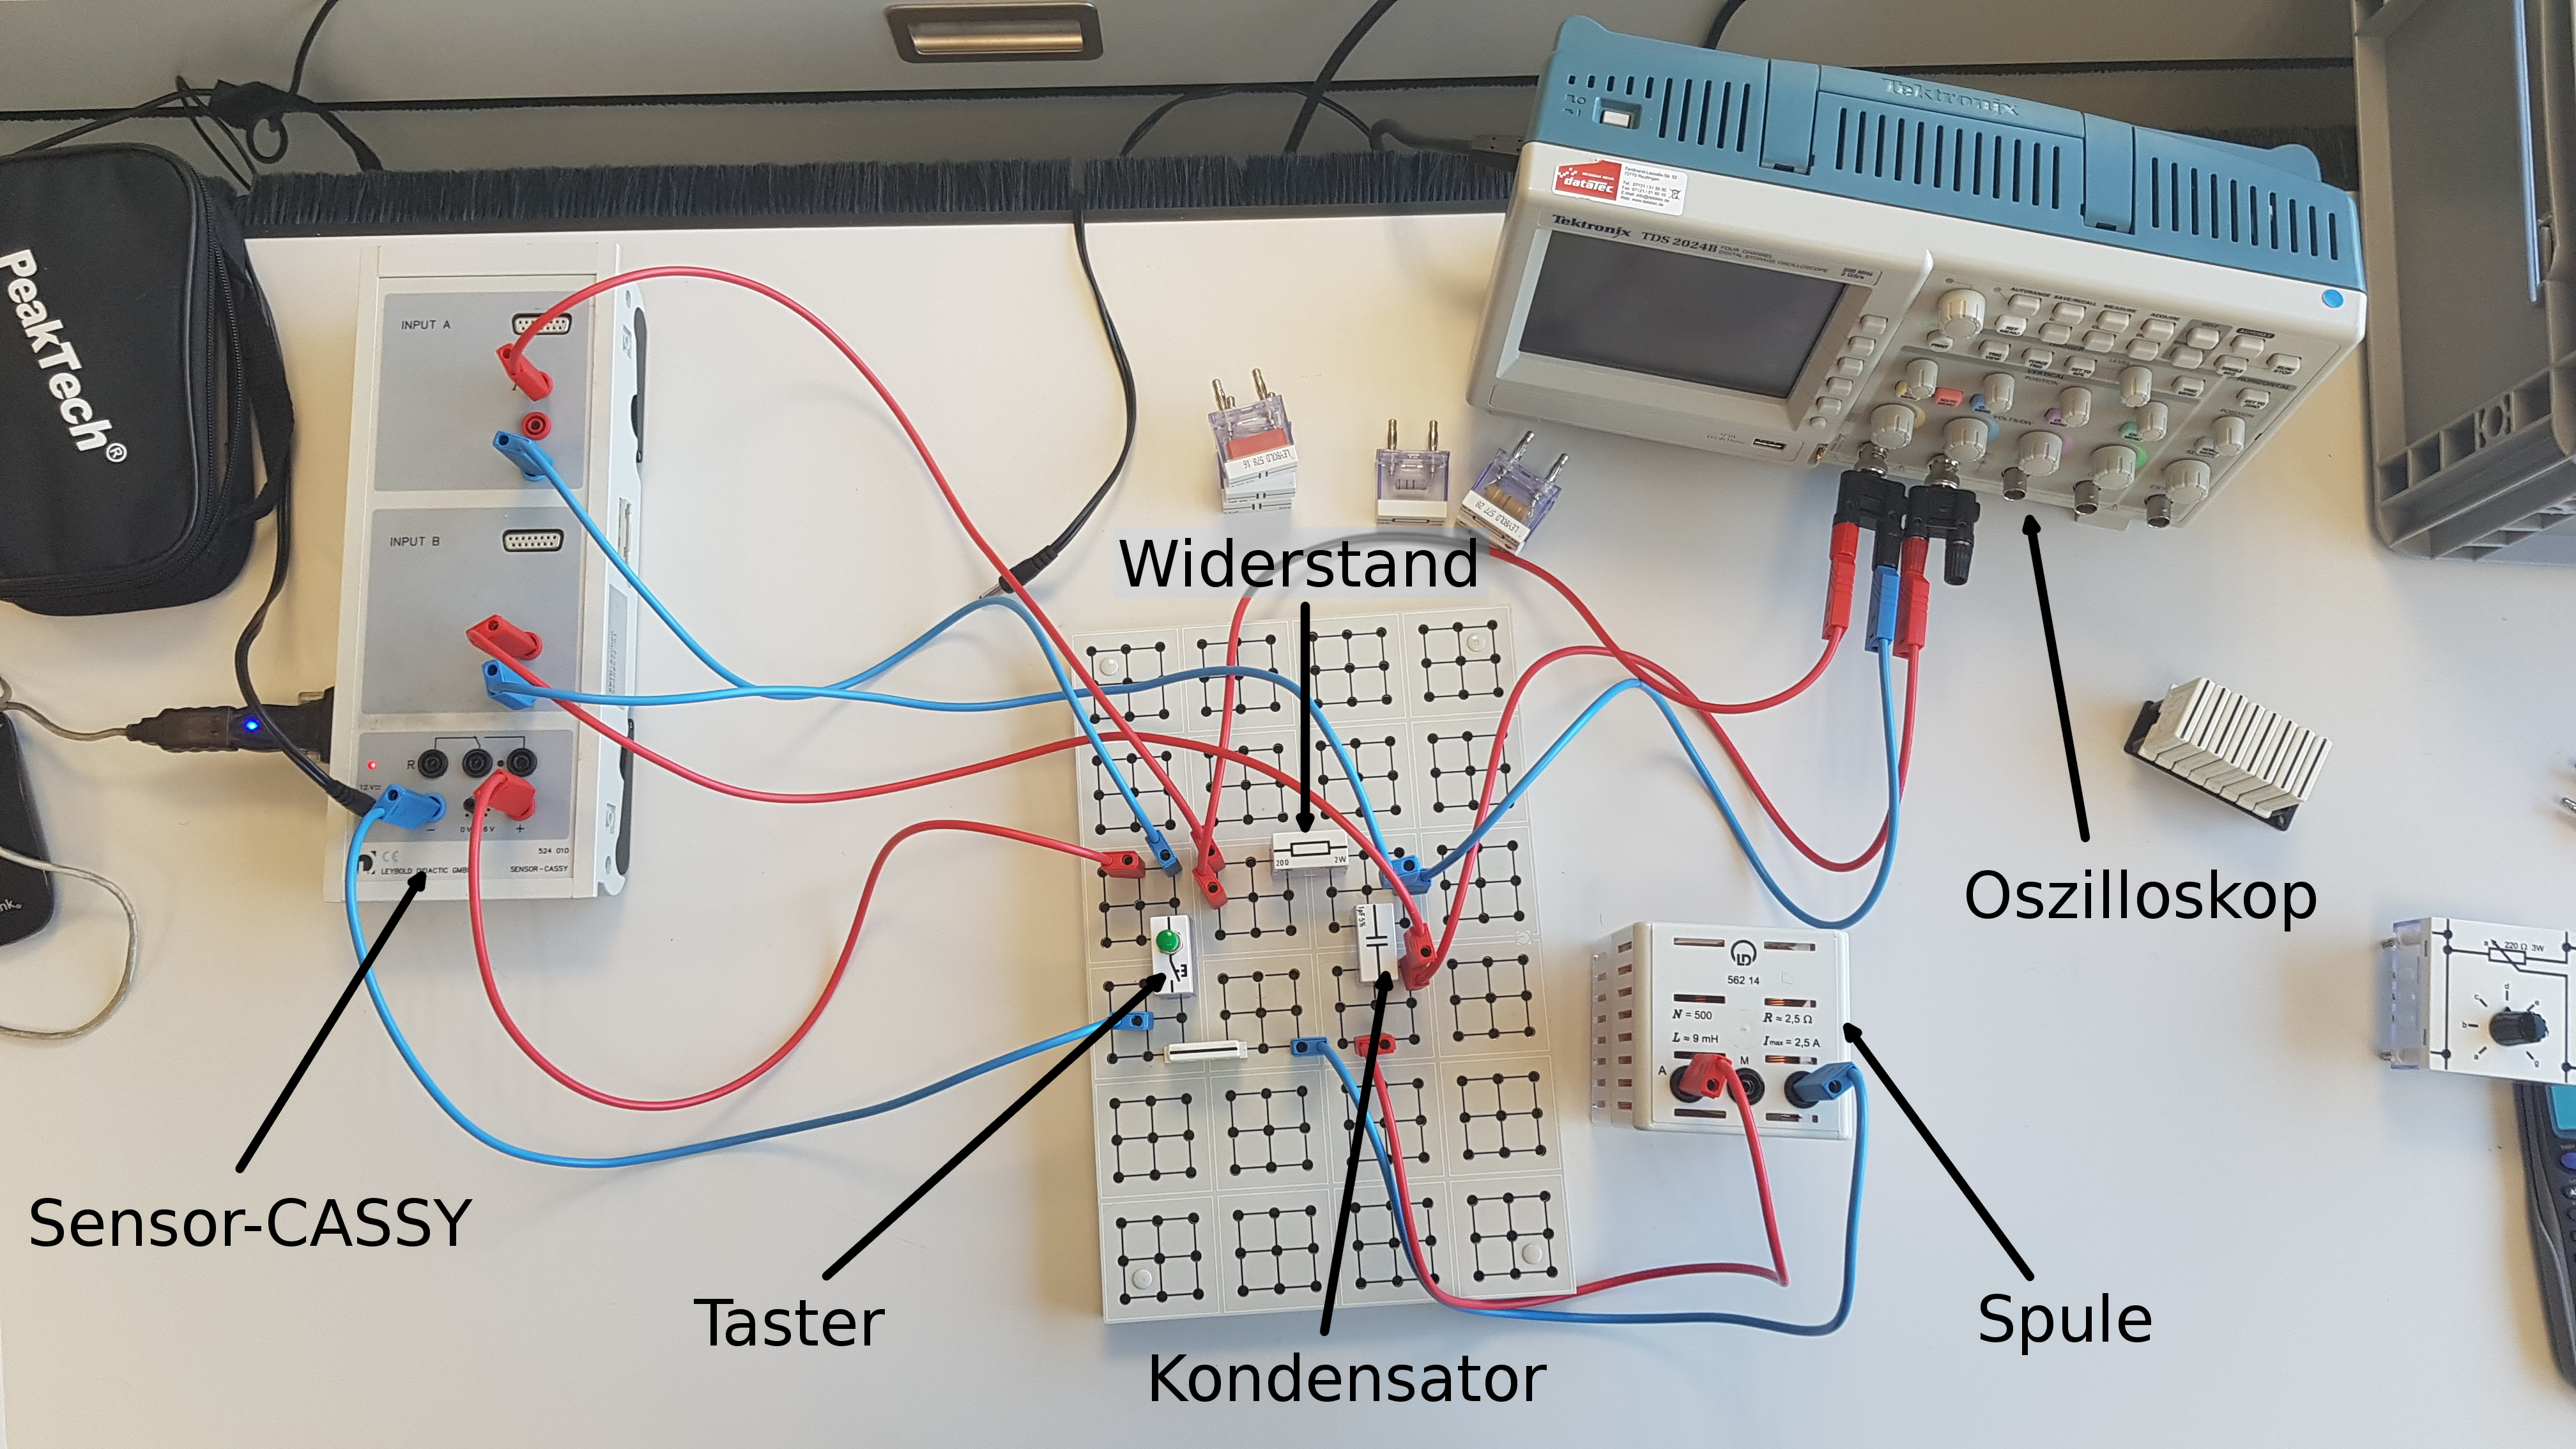
\includegraphics[width=\textwidth]{bilder/LCR_aufbau_beschriftet.jpg}
\caption{Versuchsaufbau LCR-Schwingkreis}
\label{abb:aufbau_lcr}
\end{figure}
Das Schaltbild aus Abbildung \ref{abb:schaltLCR} wird auf der Rastersteckplatte aufgebaut. Dies ist in Abbildung \ref{abb:aufbau_lcr} zu sehen. Als Spannungsquelle dient die Spannungsquelle des Sensor-CASSY. Die Spannung am Kondensator wird am Eingang B und die Stromstärke am Eingang A gemessen. Zusätzlich wird die Spannung am Kondensator am Channel 1 und die Spannung am Widerstand am Channel 2 des Oszilloskops gemessen. Die Erde liegt dabei zwischen Kondensator und Widerstand, wie im Schaltbild eingezeichnet.

\subsection{Versuchsdurchführung}



\subsection{Versuchsauswertung}

Die Rohdaten für alle verschiedenen Fälle sind in Abbildung \ref{abb:rohdaten_ska} zu sehen.

\begin{figure}[H]
\centering
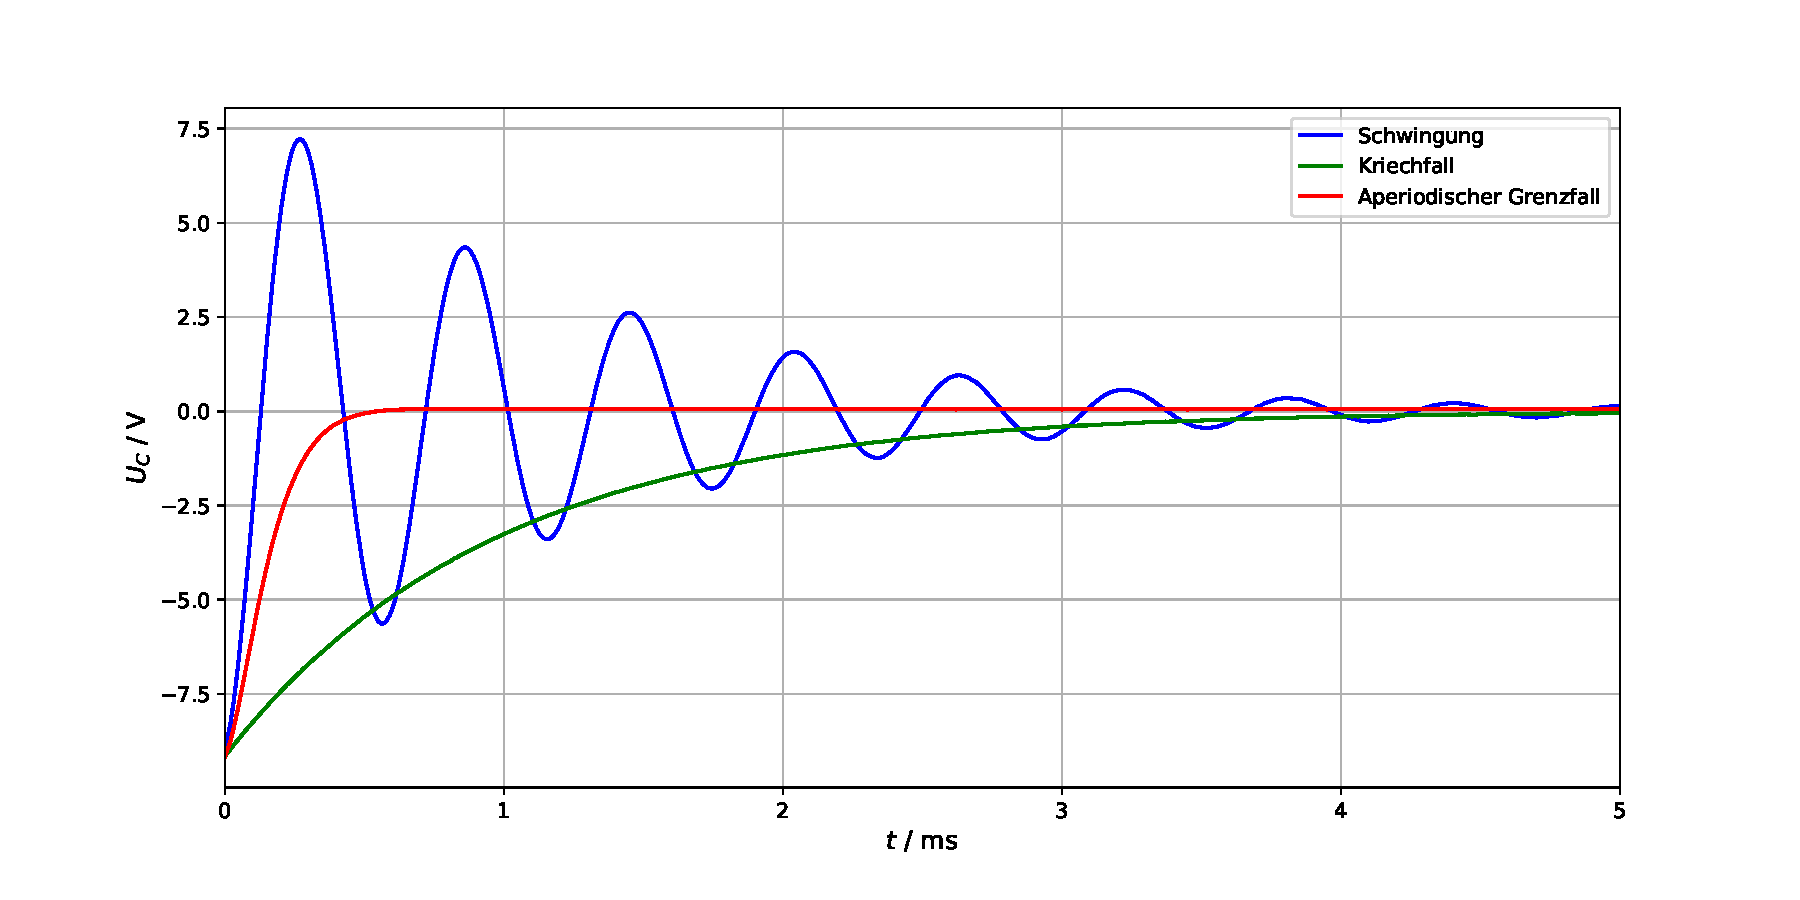
\includegraphics[width=\textwidth]{plots/rohdaten_ska.pdf}
\caption{Rohdaten mit Schwing-, Kriech- und Aperiodischem Grenzfall}
\label{abb:rohdaten_ska}
\end{figure}


\subsection{Fazit}




\section{Gekoppelte LC-Schwingkreise}


\subsection{Versuchsbeschreibung}

In diesem Versuch werden zwei Schwingkreise induktiv miteinander gekoppelt. Speziell werden hier die beiden Fundamentalschwingungen bei gleichsinniger und gegensinniger Anregung und eine Schwebung aufgezeichnet.

Für den gekoppelten Schwingkreis gelten die folgenden Differentialgleichungen
\begin{align*}
\ddot I_1 + k \ddot I_2 + \frac{1}{LC}I_1 &= 0 \\
\ddot I_2 + k \ddot I_1 + \frac{1}{LC}I_2 &= 0
\end{align*}
Dabei bezeichnet $k \in (0,1)$ die Kopplung der beiden Schwingkreise. 
Mit den sogenannten \textit{Fundamentalströmen} $I_+ = I_1 + I_2$ und $I_- = I_1 - I_2$ erhält man durch Addition bzw. Subtraktion der obigen Gleichungen und anschließendem Umformen
\begin{align*}
\ddot I_+ + \frac{1}{LC(1+k)} I_+ = 0 \\
\ddot I_- + \frac{1}{LC(1-k)} I_- = 0
\end{align*}
Daraus ergeben sich harmonische Schwingungen mit den Kreisfrequenzen 
$$\omega_+ = \frac{\omega_0}{\sqrt{1+k}} \hspace{0.2cm} \text{ und } \hspace{0.2cm} \omega_- = \frac{\omega_0}{\sqrt{1+k}}.$$
Dabei ist $\omega_0 = \frac{1}{\sqrt{LC}}$ die Kreisfrequenz der ungekoppelten Schwingung. Mithilfe der Fundamentalschwingungen lässt sich dann der Kopplungsgrad bestimmen
$$k = \frac{f_-^2 - f_+^2}{f_-^2 + f_+^2}.$$
Bei Messung einer Schwebung mit Schwebungsfrequenz $f_s$ und Frequenz der gekoppelten Schwingung $f_k$ kann man die Fundamentalschwingungen gemäß
$$f_k = \frac{f_- + f_+}{2} \hspace{0.2cm} \text{ und } \hspace{0.2cm} f_s = \frac{f_- - f_+}{2}$$
bestimmen. Aufgrund der unvermeidbaren Dämpfung der beiden Schwingkreise sind die Extrema des einen Schwingkreises gegen die Nulldurchgänge des anderen verschoben. Für Kopplungen $k < 0.2$ gilt näherungsweise für die zeitliche Verschiebung
$$\Delta t \approx \frac{1}{\omega_s} \left( \frac{\pi}{2} - \arctan\left(  \frac kR \sqrt{\frac LC}\right) \right).$$


\subsection{Versuchsaufbau}

\subsection{Versuchsdurchführung}

\subsection{Versuchsauswertung}

\subsection{Fazit}

\end{document}